
% --------------------------------------------------------------------
% This is a simple Beamer document that uses beamerthemesigma.sty
% Reading the comments should help you create a presentation even if
% you've never used Beamer before.
% --------------------------------------------------------------------
% Set our document class to Beamer
\documentclass[aspectratio=169]{beamer}

% Some packages for nice font encodings in the final PDF
\usepackage[utf8]{inputenc}
\usepackage[T1]{fontenc}

% From Jeff E
\usepackage{algo}

\usepackage{sigmastyle}

% To insert images
\usepackage{graphicx}

% Useful packages from the AMS
\usepackage{amsmath,amssymb,amsthm}

% for parse tree
\usepackage{forest}

% Package for code highlighting
\usepackage{minted}
\setminted{linenos=true, breaklines=true, breakanywhere=true, style=default}
\usemintedstyle{monokai}

% Set a title
\title{Introducing the ``lambda calculus''}

% The subtitle is generally where I'd expect you to put the week
% number, thus:
\subtitle{Week 10}
% \texorpdfstring to remove compilation warnings if you have math here

% Whoever worked on the presentation:
\author{Phil}

% A date, if you'd like.
\date{}

% An institute name, if you're so inclined
% \institute{University of Illinois Urbana-Champaign}

% Use the SIGma theme for this Beamer presentation
\usetheme{sigma}
% --------------------------------------------------------------------
% Begin document
\begin{document}

% Beamer calls each slide a "frame", defined within the environment:
% \begin{frame}
%   <frame content here>
% \end{frame}

% This frame is just the title.
\begin{frame}
\titlepage
\end{frame}

% A frame with the table of contents.
% This frame's title is "Outline".
\begin{frame}{Outline}
  \tableofcontents
\end{frame}

\begin{frame}{Updates!}
  Weekly updates: \pause
  \begin{itemize}
    \item no stickers yet :(
  \end{itemize}
\end{frame}

\section{Definitions}
\frame{\sectionpage}

\begin{frame}{Models of Computation}
    \begin{itemize}
        \item Previously we talked about \textbf{Turing machines} and \textbf{Turing completeness} \pause
        \item The \textbf{Church-Turing thesis}, proven in the 1930s by \textit{Alonzo Church} and \textit{Alan Turing}, states, roughly, that functions on natural numbers are "effectively calculable" iff a Turing machine can compute it. \pause
        \item But are there other models of computation that can "effectively calculate" numbers? Then they should be Turing complete, right?
    \end{itemize}
\end{frame}

\begin{frame}{$\lambda$ Calculus?}
    Yes! Alonzo Church's \textit{lambda calculus} looks very different from a Turing machine. But it has all of the same capabilities.
    \begin{center}
    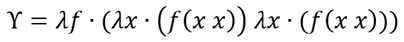
\includegraphics[width=\textwidth]{images/y_combinator.png}
    \end{center}
\end{frame}

\begin{frame}{A short definition}
    The lambda calculus looks similar to a functional programming language (really, it'd be more accurate to say that they look like the lambda calculus). We'll define a grammar to describe how to parse the language, and a very short list of operations used to "evaluate" lambda calculus expressions. \pause \\ \\
    \textbf{Remember BNFs from parsing?} Here's the lambda calculus BNF: \\
    \begin{align*}
        e \hspace{0.025in} &::= x \hspace{0.5in} \text{// variable} \\
        &\mid e \hspace{0.05in} e \hspace{0.55in} \text{// function application} \\
        &\mid \lambda x \hspace{0.05in} . \hspace{0.05in} e \hspace{0.35in} \text{// function definition} \\
    \end{align*}
\end{frame}

\begin{frame}{Short Examples}
    \begin{itemize}
        \item \underline{\textbf{x}} is just a variable x.
        \item \underline{\textbf{y}} is just a variable y. Are these programs equivalent? \pause (yes)
        \item \underline{\textbf{x y}} is an application of "x" to "y". Both "x" and "y" are variables. \pause
        \item \underline{\textbf{$\lambda$ x . x}} defines a function (sometimes called abstraction). It "takes x" and its body is the expression "x". what kind of function is this? \pause (looks like the identity function)
    \end{itemize}
\end{frame}

\begin{frame}{Parentheses}
    \begin{itemize}
        \item How do we parse \underline{\textbf{$\lambda$ x . $\lambda$ y . x y x}} ? \pause
        \begin{itemize}
            \item Assume function body extends as far right as possible
            \item Successive applications are left associative. \pause
        \end{itemize}
        \item Equivalent to \underline{\textbf{$\lambda$ x . ($\lambda$ y . (x y) x)}}
    \end{itemize}
\end{frame}

\begin{frame}{}
    \begin{center}
        {\color{sigma@mainblue} \LARGE Questions?}
    \end{center}
\end{frame}

\section{Semantics}
\frame{\sectionpage}

\begin{frame}{$\beta$ Reduction}
    \begin{itemize}
    \item quick: \textbf{value} $::= \lambda x . e$
    \item Here's the first operation we'll define... it's how to evaluate an expression: \pause
    \begin{itemize}
        \item \textbf{($\lambda$ x . e) v $\to$ e $[$ v / x $]$}
        \item in words: if we have a \textit{function} applied to a \textit{value}, then
        \item it is "$\beta$ equivalent" to a \textit{substitution:}
        \item where we take "e" and replace all "x" with "v". \pause
    \end{itemize}
    \item Here's an example: 
    \begin{itemize}
        \item ($\lambda$ x . x) ($\lambda$ y . z)   $\to$ x   $[$ ($\lambda$ y . z) / x $]$ \pause
        \item x $[$ ($\lambda$ y . z) / x $]$   $\to$   \underline{\textbf{$\lambda$ y . z}}
    \end{itemize}
    \end{itemize}
\end{frame}

\begin{frame}{$\beta$ Reduction Rules}
In general, when simplifying an application: $\beta$ reduce the left side, then the right side \textit{if the left side is a value}, then if both sides are values, $\beta$ reduce the application.
\begin{align*}
    e_1 \hspace{0.1in} e_2 & \to e'_1 \hspace{0.1in} e_2 \hspace{0.2in} \text{ only if $e_1 \to e_1'$} \\
    v \hspace{0.1in} e_2 & \to v \hspace{0.1in} e_2' \hspace{0.2in} \text{ only if $e_2 \to e_2'$} \\
\end{align*}
\end{frame}

\begin{frame}{}
    \begin{center}
        {\color{sigma@mainblue} \LARGE Questions?}
    \end{center}
\end{frame}

\begin{frame}{Now, some linguistics}
    Let's look at some sentences! \\
    \begin{itemize}
    \item Susie lost her book. \pause
    \item Susie lost \underline{her} book. \pause
    \item Susie lost \underline{her} book. \textit{Alice had a book.} (whose book did Susie lose?) \pause
    \item Susie lost \underline{her own} book. (oh, Susie lost her own book)
    \end{itemize}
\end{frame}

\begin{frame}{Free and Bound Variables}
    \begin{itemize}
    \item What is "y" here? \underline{\textbf{$\lambda$ x . $\lambda$ y . y}}
    \item What is "x" here? \underline{\textbf{$\lambda$ x . $\lambda$ y . x}} \pause
    \item \textbf{Bound variables} refer to the argument of the function they are in.
    \item \textbf{Free variables} refer to a variable declared outside the function body.
    \end{itemize}
\end{frame}

\begin{frame}{$\alpha$ Renaming}
Let's say we have \underline{($\lambda$ x . y)} and want to substitute y with "x". How do we do that? \pause \\

\begin{itemize}
\item What kind of variable is y in \underline{($\lambda$ x . y)} ? \pause (free)
\item When we are substituting in new values for free variables, we have to avoid naming conflicts.
\item $\alpha$ equivalent - we can rename variables as long as it doesn't change the meaning of the program. 
\end{itemize}

We change the expression to \underline{($\lambda$ z . y)} and then substitute "x" for "y" to get \underline{($\lambda$ z . x)}. Great!
\end{frame}

\begin{frame}{Exercise}
    Let's try a more complex one, try reducing this expression (finding its normal form):
    \begin{itemize}
        \item (($\lambda$ x. $\lambda$ y. x y) ($\lambda$ y . y)) ($\lambda$ z . z) \pause
        \item ($\lambda$ w. ($\lambda$ y . y) w) ($\lambda$ z . z)
        \item ($\lambda$ y . y) ($\lambda$ z . z)
        \item ($\lambda$ z . z)
    \end{itemize}
\end{frame}

\section{Abstract Data Types}
\frame{\sectionpage}

\begin{frame}{Computation?}
    How do we actually compute in lambda calculus? \pause \\
    Well, we have to create some \textbf{abstract data types}. We'll define what a data type is in lambda calculus, and then define functions that return expressions matching our data types. \pause \\

    Let's define booleans:
    \begin{itemize}
    \item True $::= \lambda x. \lambda y. x$ \\
    \item False $::= \lambda x. \lambda y. y$ \\
    \end{itemize}

    Can you write a lambda calculus function defining the conditional? (a function, given a boolean, P, and Q, returns either P or Q) \\

    What about OR (a function, given two booleans, returns the OR of the two) (you can use "true" or "false" in your answer)
\end{frame}

\begin{frame}{Computation Answers}
Conditional: \pause
\begin{itemize}
\item $\lambda c . \hspace{0.02in} \lambda p . \hspace{0.02in} \lambda q . \hspace{0.05in} c\hspace{0.05in} p\hspace{0.05in} q$ \pause
\item explanation: our boolean "takes in" two arguments. if its true, it returns the first input, if its false, it returns the second, by definition.
\end{itemize}
OR gate: \pause
\begin{itemize}
\item $\lambda a . \hspace{0.02in} \lambda b . \hspace{0.05in} a \hspace{0.05in} \text{true} \hspace{0.05in} b$
\item this should remind you of \textit{short circuit evaluation} if you've learned that about programming languages. if A, then true, else return B.
\end{itemize}
\end{frame}

\section{Y Combinator}
\frame{\sectionpage}

\begin{frame}{Something's missing...}
Does lambda calculus support recursion? \pause

Let's look at the Y combinator: $Y = \lambda f ((\lambda x. f (x \hspace{0.05in} x)) (\lambda x. f (x \hspace{0.05in} x)))$. \\ What if we apply a function $g$ to this? \\ \\
$Y\hspace{0.05in} g = $
\begin{itemize}
\item Substituting g for f:
\item $Y\hspace{0.05in} g = (\lambda x.\hspace{0.05in} g\hspace{0.05in} (x\hspace{0.05in} x))\hspace{0.05in} (\lambda x.\hspace{0.05in} g\hspace{0.05in} (x\hspace{0.05in} x))$ \pause
\item Applying:
\item $Y\hspace{0.05in} g = g\hspace{0.05in} ((\lambda x.\hspace{0.05in} g\hspace{0.05in} (x\hspace{0.05in} x))\hspace{0.05in} (\lambda x.\hspace{0.05in} g\hspace{0.05in} (x\hspace{0.05in} x)))$
\item $Y\hspace{0.05in} g = g\hspace{0.05in} (Y\hspace{0.05in} g)$
\end{itemize}
\end{frame}

\begin{frame}{Y Combinator}
What is a combinator?
\begin{itemize}
\item a "higher-order" function that returns a fixed point of its argument function.
\item "higher-order" means it takes in a function as an argument. For example a sort function can take in a function telling you how to order the elements.
\item fixed point of a function f (call it fix f) means fix f = f(fix f) = f(f(fix f)) = ...
\end{itemize}
\pause
Y Combinator is just one example. There are actually infinitely many combinator functions possible in the lambda calculus.
\end{frame}

\begin{frame}{Y Combinator Useful for?}
Remember, you \textbf{can't} refer to a function within the function in lambda calculus (put differently, all functions are anonymous, unnameable to themselves) \\ \pause

But you \textbf{can} use the Y combinator to pass a function to itself... thereby always giving it a reference with which to call itself! \\ \pause

Example: factorial = $\lambda$ f . $\lambda$ n . cond (is\_zero n) (1) (mul n (f (pred n)) \\ \pause
Key point: Y factorial 2 = factorial (Y factorial) 2 (!!)

\end{frame}

\font\eightss=cmssq8
\font\eightssi=cmssqi8
\newcommand\quoteAuthorDate[3]{\begingroup
  \baselineskip 10pt
  \parfillskip 0pt
  \interlinepenalty 10000 % not needed in example
  \leftskip 0pt plus 40pc minus \parindent
  \let\rm=\eightss
  \let\sl=\eightssi
  \everypar{\sl}#1\par
  \nobreak\smallskip
  \noindent\rm--- #2\unskip\enspace(#3)\par
  \endgroup}
% If someone can figure out how to horizontally center this and make the text bigger that'd be cool
\begin{frame}
    \textit{Next time...}
    \begin{center}
        \item \quoteAuthorDate{We toast the Lisp programmer who pens his thoughts within nests of parentheses.}{ALAN PERLIS}{1984}
    \end{center}
\end{frame}

\end{document}